\documentclass{beamer}

\usetheme{Copenhagen}
%% \usenavigationsymbolstemplate{}
\setbeamertemplate{navigation symbols}{}
%% \usecolortheme[rgb={0.4,0.5,0.4}]{structure}
\usepackage{color}
\usepackage{listings}
% \usepackage[T1]{fontenc}
% \usepackage{libertine}
\usepackage[spanish]{babel}
\usepackage[utf8]{inputenc}
\usepackage{graphicx}
\usepackage{verbatim}
\usepackage{hyperref}
%\usepackage{wrapfig}
\usepackage{siunitx}
\usepackage[version=3]{mhchem}

\graphicspath{ 
	{../../FEM_termico/celula/scripts/itvs/}
	{../../FEM_termico/celula/scripts/curvas/}
	{../../FEM_termico/celula/scripts/poros/}
	{../../FEM_termico/AutoMesh2D/grande/}
}

\title{Electroporación celular}
      
\author{Mauricio Alfonso}
\institute{DC - FCEyN - UBA}
%\date[11.2013]{SegInf, 2c - 2013}

\begin{document}
	\newcommand{\h}{\ce{H^+}}
	\newcommand{\oh}{\ce{OH^-}}
	\newcommand{\na}{\ce{Na^+}}
	\newcommand{\cl}{\ce{Cl^-}}
	\newcommand{\kvm}{$\si{\kilo\volt\per\metre}$}
	\newcommand{\usec}{$\si{\micro\second}$}

	\begin{frame}
		\titlepage
	\end{frame}

	\section{Introducción}
		\frame{
			\begin{itemize}
				\item Una célula esférica de entre 10 y 50 \si{\micro\metre} de radio
				\item Dos electrodos que generan un pulso de 20 \si{\milli\second} de entre 40 y 200 \kvm
				\item Se estudia la generación de poros en la membrana celular y el ingreso de \h, \oh, \na{} y \cl{} a la célula.
				
			\end{itemize}
		}
	
	\section{Mallado}
		\frame{
			\begin{itemize}
				\item Coordenadas cilíndricas (2D)
				\item Elementos cuadrilaterales
				\item Programa AutoMesh2D para generar mallas
				\item 2 mallas diferentes: una de 1930 elementos y otra de 7439 elementos
			\end{itemize}
		}
		
		\frame{
			\begin{center}
				%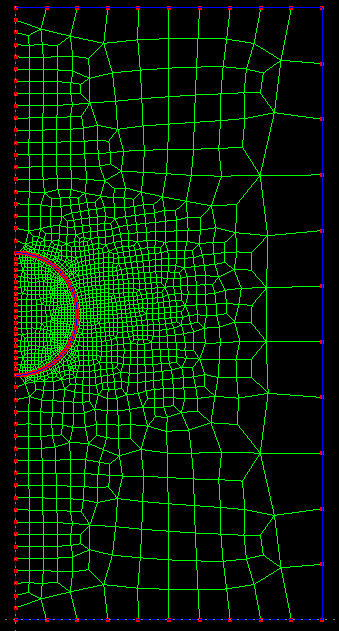
\includegraphics[keepaspectratio,width=.6\textwidth]{grande} \\
				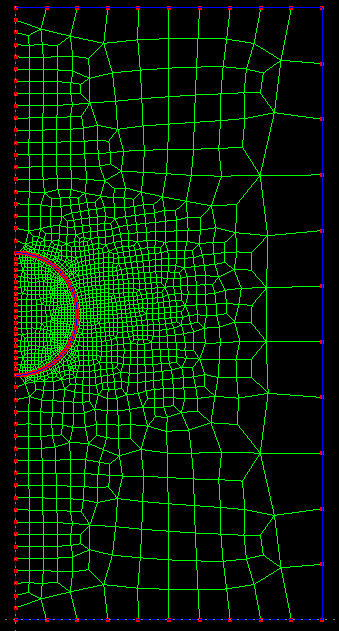
\includegraphics[keepaspectratio, height = \textheight]{grande} \\
				%Ejemplo de malla
			\end{center}
		}
	
		\frame{
			\begin{center}
				%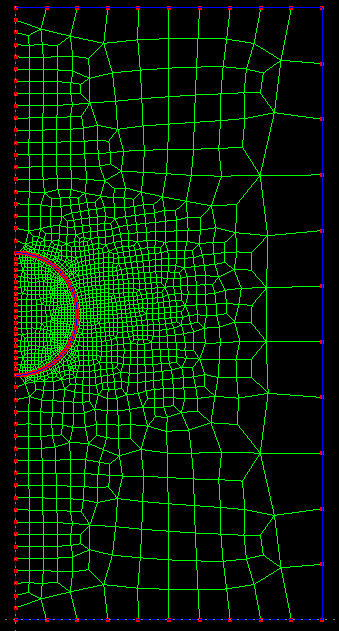
\includegraphics[keepaspectratio,width=.6\textwidth]{grande} \\
				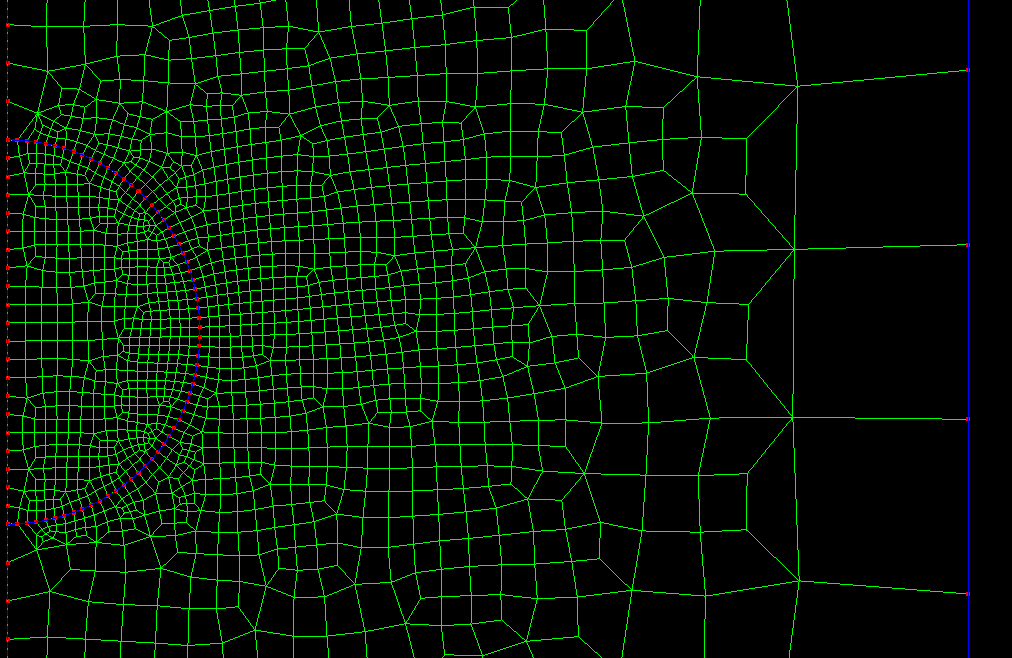
\includegraphics[keepaspectratio, height = 0.95\textheight]{grande2} \\
				%Ejemplo de malla
			\end{center}
		}

	\section{Potencial Eléctrico}
		\frame{
			Potencial eléctrico:
			\begin{center}
				$\nabla \sigma_{elem} \cdot (\nabla \phi) = 0$
			\end{center}
			Condiciones de borde de Dirichlet en los electrodos y Neumann en los otros bordes.\\
			
			El potencial transmembrana (ITV) debería aproximarse a:
			\begin{center}
				$V^{\theta} = 1.5 E cos (\theta)$
			\end{center}
		}
		
		\frame{
			Capacitancia de la membrana:
			FALTA ESTO!!!!
		}
		
	%	ACÁ PODRÍA IR UN DELAUNAY DE POTENCIAL O CAMPO!!!
	
	\section{Generación de poros}
		\frame{
			Generación de poros (densidad):
			\begin{center}
				$\frac{\partial N}{\partial t} = \alpha_c e^{(V_m/V_{ep})^2} \left( 1 - \frac{N}{N_0 e^{q \left(V_m/V_{ep} \right) ^2}} \right)$
			\end{center}
			$N$ es la densidad de poros en un determinado tiempo y posición de la membrana celular, $\alpha_c$ es el coeficiente de creación de poros, $V_m$ es el potencial transmembrana, $V_{ep}$ es el voltaje característico de electroporación, $N_0$ es la densidad de poros en equilibrio (cuando $V_m = 0$) y $q$ es una constante igual a $(r_m / r*)^2$, donde $r_m$ es el radio de mínima energía para $V_m = 0$ y $r*$ es el radio mínimo de los poros.\\
			
			La densidad depende del ángulo (no es constante en toda la superficie).
		}
	
		\frame{
			Radio de los poros:
			\begin{center}
				$\frac{\partial r}{\partial t} = \frac{D}{kT} \left( \frac{V_m^2 F_{max}}{1+r_h / (r+r_a)} + \frac{4 \beta}{r} \left(\frac{r_*}{r}\right)^4 - 2 \pi \gamma + 2 \pi \sigma_{\textrm{\tiny eff}} r\right) ,$
			\end{center}
			
			\begin{center}
				$ \textrm{con } \sigma_{\textrm{\tiny eff}} = 2 \sigma^\prime - \frac{2 \sigma^\prime - \sigma_0}{(1 - A_p / A)^2}	$
			\end{center}		
			
			Se aplica a cada poro por separado. Modela como crece el radio de los poros, y como se vuelven a sellar si baja el ITV.
			
			El primer término corresponde a la fuerza eléctrica inducida por el potencial transmembrana, el segundo a la repulsión estérica, el tercero a la tensión de línea que actúa en el perímetro del poro y el cuarto a la tensión superficial de la célula.
		}
	
		\frame{
			Donde $r$ es el radio de un poro, $D$ es el coeficiente de difusión para los poros, $k$ es la constante de Boltzmann, $T$ la temperatura absoluta, $V_m$ el potencial transmembrana, $F_{max}$ la máxima fuerza eléctrica para $V_m$ de 1V, $r_h$ y $r_a$ son constantes usadas para la velocidad de advección, $\beta$ es la energía de repulsión estérica, $\gamma$ es la energía del perímetro de los poros, y $\sigma_{\textrm{\tiny eff}}$ es la tensión efectiva de la membrana, $\sigma^\prime$ es la tensión de la interfase hidrocarburo-agua, $\sigma_0$ es la tensión de la bicapa sin poros, $A_p$ es la suma de las áreas de todos los poros en la célula, y $A$ es el área de la célula. 
		}	
	
	\section{Transporte}
		\frame{
			Transporte de especies: Nernst-Planck
			\begin{center}
				$\frac{\partial C_i}{\partial t} = \nabla \cdot \left( D_i \nabla C_i + D_i z_i \frac{F}{R T} C_i \nabla \phi \right)$
			\end{center}
			$C_i$ es la concentración de la especie $i$, $D_i$ el coeficiente de difusión de la especie $i$, $z_i$ la valencia de la especie $i$, $F$ la constante de Faraday, $R$ la constante de los gases y $T$ la temperatura.					
		}

	\section{Implementación}
		\frame{
			\begin{block}{Implementación}
				\begin{itemize}
					\item Métodos de elementos finitos para potencial eléctrico (ecuación de Poisson) y transporte de especies
					\item Diferencias finitas para generación y evolución de poros
					\item Implementado en \texttt{C++}
					\item Librería Eigen para resolver sistemas de ecuaciones
					\item Descomposiciones Cholesky (para Poisson) y Bi-gradientes conjugados estabilizados (para transporte)
					\item OpenMP para acelerar llenado de matrices (Poisson) y resolución en transporte
				\end{itemize}
			\end{block}
		}

	\section{Resultados}
		\frame{
			
		}	
		
	\section{Trabajo Pendiente}
	

	\section{Herramientas y ambiente}
	    \frame{
    	    \begin{itemize}
        	    \item Android SDK\footnote{\url{https://developer.android.com/sdk/index.html}}
                \item Genymotion Android emulator\footnote{\url{http://www.genymotion.com}}
                \item Eclipse plugins para ambas cosas.
            \end{itemize}
        }
        
        \section{Animal}

        \frame{
            \begin{block}{Descripci\'on del malware}
                Animal es un malware de Android que busca fotos en la tarjeta SD de la v\'ctima y las sube a un servidor.
            \end{block}
            \begin{block}{Permisos requeridos}
                El \'unico permiso que requiere es acceso a internet (\texttt{android.permission.INTERNET}).
            \end{block} 
        }

        \subsection{Information leakage / control}
        \frame{
            \begin{block}{C\'omo funciona?}
                    \begin{enumerate}
                        \item Abre una actividad\footnote{\url{http://developer.android.com/reference/android/app/Activity.html}} que busca archivos de im\'agenes en los directorios \texttt{DCIM/Camera}, \texttt{Pictures} y \texttt{Downloads} de la tarjeta SD del celular. 
                        \item Lanza conexiones \texttt{HTTP} sobre las  que se env\'ian los archivos a nuestro servidor (\texttt{Servercito}).
                        \item La direcci\'on de \texttt{Servercito} est\'a hardcodeada en el c\'odigo y las im\'agenes se convierten a base64 y se mandan usando los par\'ametros de url de un POST HTTP. 
                    \end{enumerate}
            \end{block}
        }

        \frame{
            \begin{itemize}
                \item (Sinatra rb) restfull 
                    \begin{item}
                    \item distribuible
                    \item facil de mantener
                    \item extensible
                    \end{item}
                \item Operaciones GET y POST
                    \begin{itemize}
                        \item obtener contactos, fotos, etc
                        \item pushear comandos
                        \item dormirse, despertarse ?
                    \end{itemize}
                \item 
                    
            \end{itemize}
    }

        \frame{
            \begin{block}{Problemas que encontramos}
                    Intentamos en principio subir las fotos en base 64 a pastebin y poner una ``clave'' como nombre de las subidas, para poder encontrarlas con facilidad de manera an\'onima sin tener que exponer la direcci\'on de nuestro servidor, pero nos encontramos con 2 limitaciones importantes de pastebin: 
                    \begin{itemize}
                        \item Un l\'imite de tamaño de 0.5 MB nos limita a fotos muy chicas o a achicar las fotos existentes                      
                        \item Un l\'imite de 10 subidas por d\'ia.
                    \end{itemize}
            \end{block}
        }

%        \frame{
%pepe
%\begin{lstlisting}
%#!/usr/bin/ruby
%require 'sinatra'
%get '/contacts' do | res| ...
%post '/upload' do ...
%post '/key' do ...
%
%\end{lstlisting}
%
%        }


        \frame{
            \begin{block}{Mejoras a\'un no implementadas}
                    \begin{itemize}
                        \item Camuflar la aplicaci\'on para que aparente ser bien intencionada. Actualmente solo muestra una pantalla en blanco. $\rightarrow$ Podr\'iamos simular que se produjo un error y la aplicaci\'on no funciona, mientras sigue subiendo las fotos en segundo plano.
                        \item Si la v\'ictima no est\'a conectado a una red wi-fi $\rightarrow$ quedarse esperando y subir las fotos cuando s\'i lo est\'e (en segundo plano).
                        \item Buscar im\'agenes en todo el \'arbol de directorios, no s\'olo las carpetas t\'ipicas de fotos (la v\'ictima podr\'ia guardarlas en cualquier lado.)
                        \item Filtrar fotos por tamaño o nombre, de manera de subir solo aquellas que aparenten haber sido sacadas con la c\'amara del celular, y no todas las im\'agenes que se encuentren.
                    \end{itemize}
            \end{block}
        }
        
        
        \section{Animalazo}
        
        \frame{
            \begin{block}{Descripci\'on del malware}
                Animalazo es un malware de Android que roba los contactos de la v\'ctima y los sube a un servidor.
            \end{block}
            \begin{block}{Permisos requeridos}
                El \'unico permiso que requiere es acceso de lectura a la los contactos (\texttt{android.permission.READ\_CONTACTS}).
            \end{block} 
        }

        \frame{
            \begin{block}{C\'omo funciona?}
                    \begin{enumerate}
                        \item Una aplicaci\'on inofensiva invita al usuario a pelear por salvar a los animales, mostrando dos perritos corriendo.
                        \item Cuando el usuario hace click en el bot\'on para ``ayudar'':
                        \begin{itemize}
                            \item Se leen los contactos y se encodean en base64.
                            \item se crea un Intent\footnote{\url{http://developer.android.com/reference/android/content/Intent.html}} que abre un browser como si se estuviese visitando una p\'agina.
                            \item Se hace un GET a un server controlado por el atacante, enviando por los par\'ametros del GET los contactos encodeados (hay limitaciones de tama\~no)
                            \item El server malicioso responde con un Redirect (302) a google, como si nada hubiera pasado.
                        \end{itemize}
                    \end{enumerate}
            \end{block}
        }

        \frame{
            \begin{block}{Problemas que encontramos}
                    A veces la aplicaci\'on no enviaba los contactos, pensamos que tenia cacheada la URL del Intent. Despu\'es nos dimos cuenta que los distintos estados de la aplicaci\'on eran relevantes: \texttt{onCreate()}, \texttt{onStart()}, \texttt{onResume()}. Afinando mejor pudimos entender cual era el problema.
            \end{block}
        }

        \frame{
            \begin{block}{Mejoras a\'un no implementadas}
                    \begin{itemize}
                        \item Limitacion en el tama\~no de los URIs utilizados para extraer la informaci\'on. Aunque no est\'a definido este l\'imite de manera expl\'icita en el RFC2616\footnote{\url{http://www.faqs.org/rfcs/rfc2616.html}} hay limitaciones en las implementaciones.
                    \end{itemize}
            \end{block}
        }

        
        \section{Animal Keyboard + FunWithAnimals}

        \frame{
            \begin{block}{Descripci\'on del malware}
                \emph{Animal Keyboard} es un teclado de Android que ofrece un tab de emoticones para incentivar a los usuarios a instalarlo. No tiene ning\'un permiso extra, por lo que por s\'i solo es inofensivo. \emph{Al combinarse con la instalaci\'on de la aplicaci\'on FunWithAnimals, ambas act\'uan como keylogger mediante IPC}. 
            \end{block}
            \begin{block}{Permisos requeridos}
                \begin{itemize}
                    \item \texttt{android.permission.BIND\_INPUT\_METHOD} para el teclado (como cualquier otro)
                    \item \texttt{android.permission.INTERNET} para FunWithAnimals.\\ 
                    {\small Al registrar un teclado nuevo, Android advierte que \'este podr\'ia robarse tu informaci\'on. Por esto  muchas aplicaci\'ones de este tipo no incluyen permisos de internet para generar m\'as confianza\footnote{\url{http://cdn.cultofandroid.com/wp-content/uploads/2013/02/light\_flow\_1.jpg})}}.
                \end{itemize}
            \end{block} 
        }


\end{document}
